\chapter{Ensayos y resultados}

\label{Chapter4}

En este capítulo se detallan los ensayos realizados al sistema completo y los resultados obtenidos durante las pruebas de funcionamiento.

\section{Banco de pruebas}

El sistema consta físicamente de 2 tipos de componentes, nodos y servidor. El servidor posee a su vez la aplicación en el frontend y el backend con los módulos. También el sistema posee 2 tipos de nodos, control de calefacción y de iluminación.

Para ensayar el nodo de temperatura se utilizaron los materiales que lo componen que se muestran en la figura \ref{fig:31}.

\begin{figure}[h]
\centering
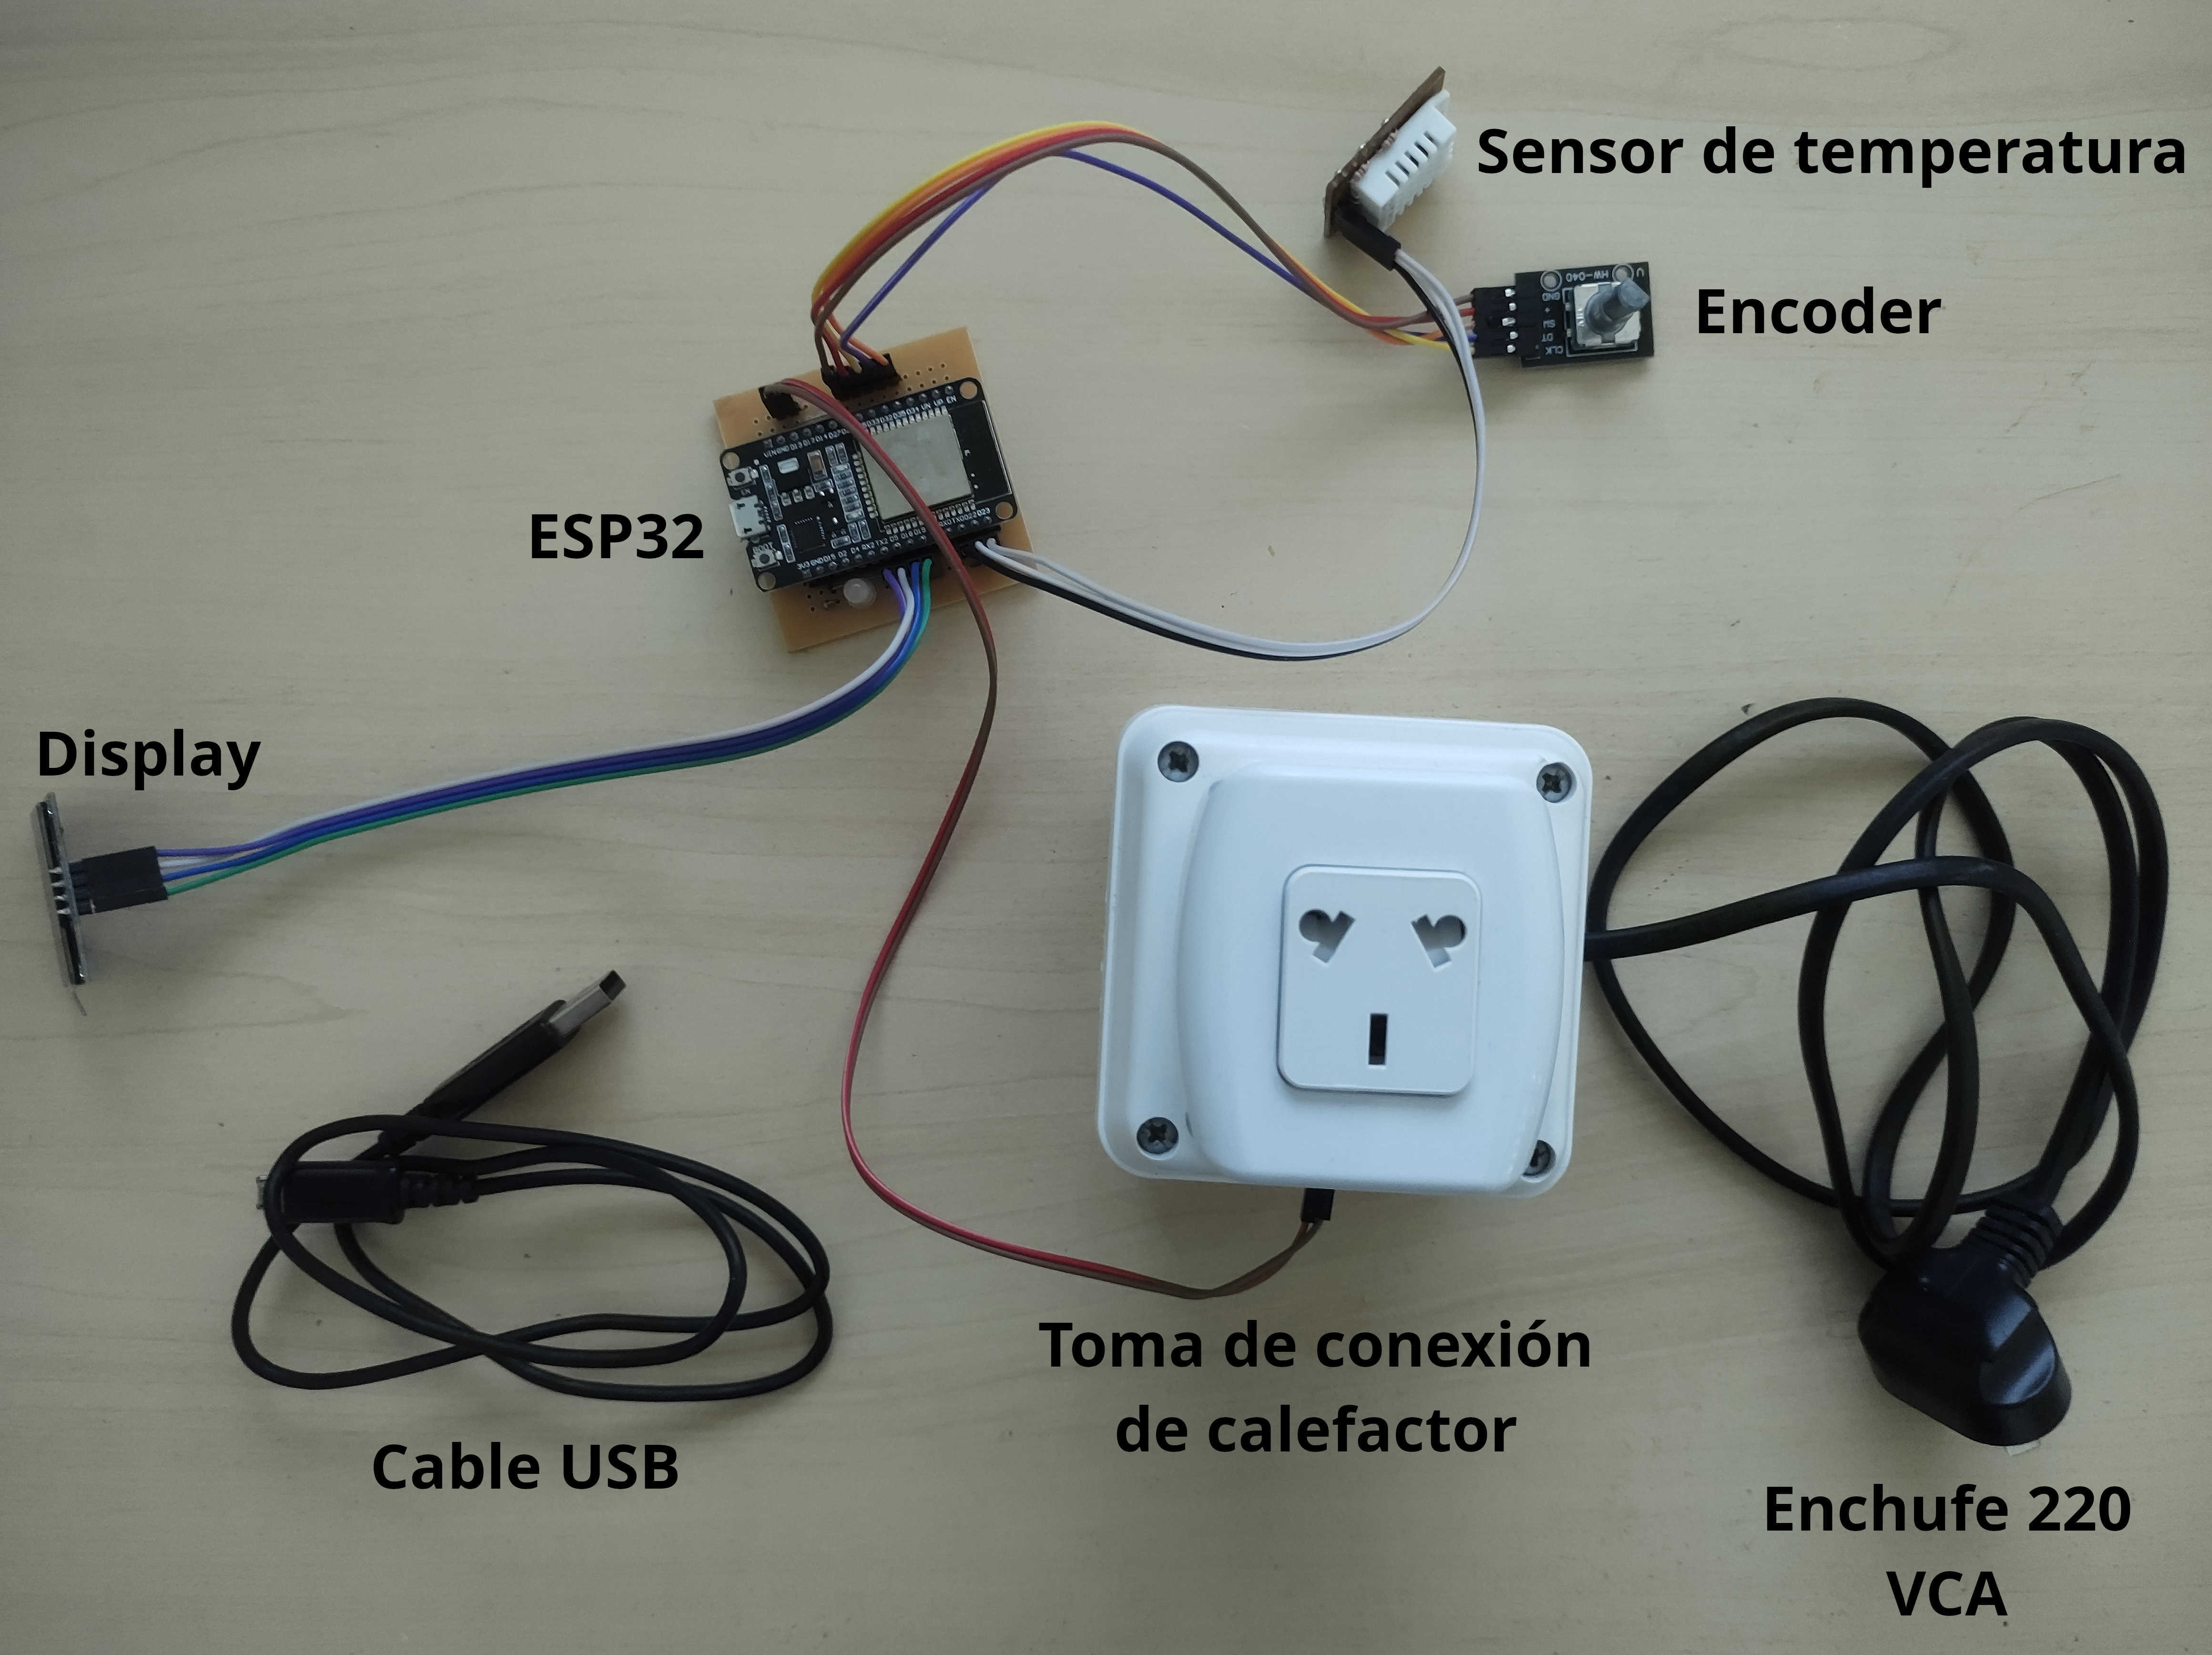
\includegraphics[scale=0.06]{Figura 31 - Nodo temperatura.jpg}
\caption[Nodo temperatura]{Componentes del nodo de temperatura.}
\label{fig:31}
\end{figure}

Se puede observar la placa ESP32 montada sobre la placa de conexiones, el display, encoder, sensor de temperatura y una caja estanca con una conexión de toma corriente para conectar la estufa a encender. Esta caja además posee un cable para conectar a 220 VCA para alimentar la estufa y que funcione como un interruptor. Cabe aclarar que en modo automático el control de temperatura funciona con una histéresis de 1 grado, por lo que al setear la temperatura en un valor determinado, el control va a apagar la salida cuando la temperatura sobrepase por 1 grado al set-point y la va a encender cuando esté 1 grado por debajo de este valor.

Para ensayar el nodo de dimerización se utilizaron los materiales que lo componen que se muestran en la figura \ref{fig:32}.

\begin{figure}[h]
\centering
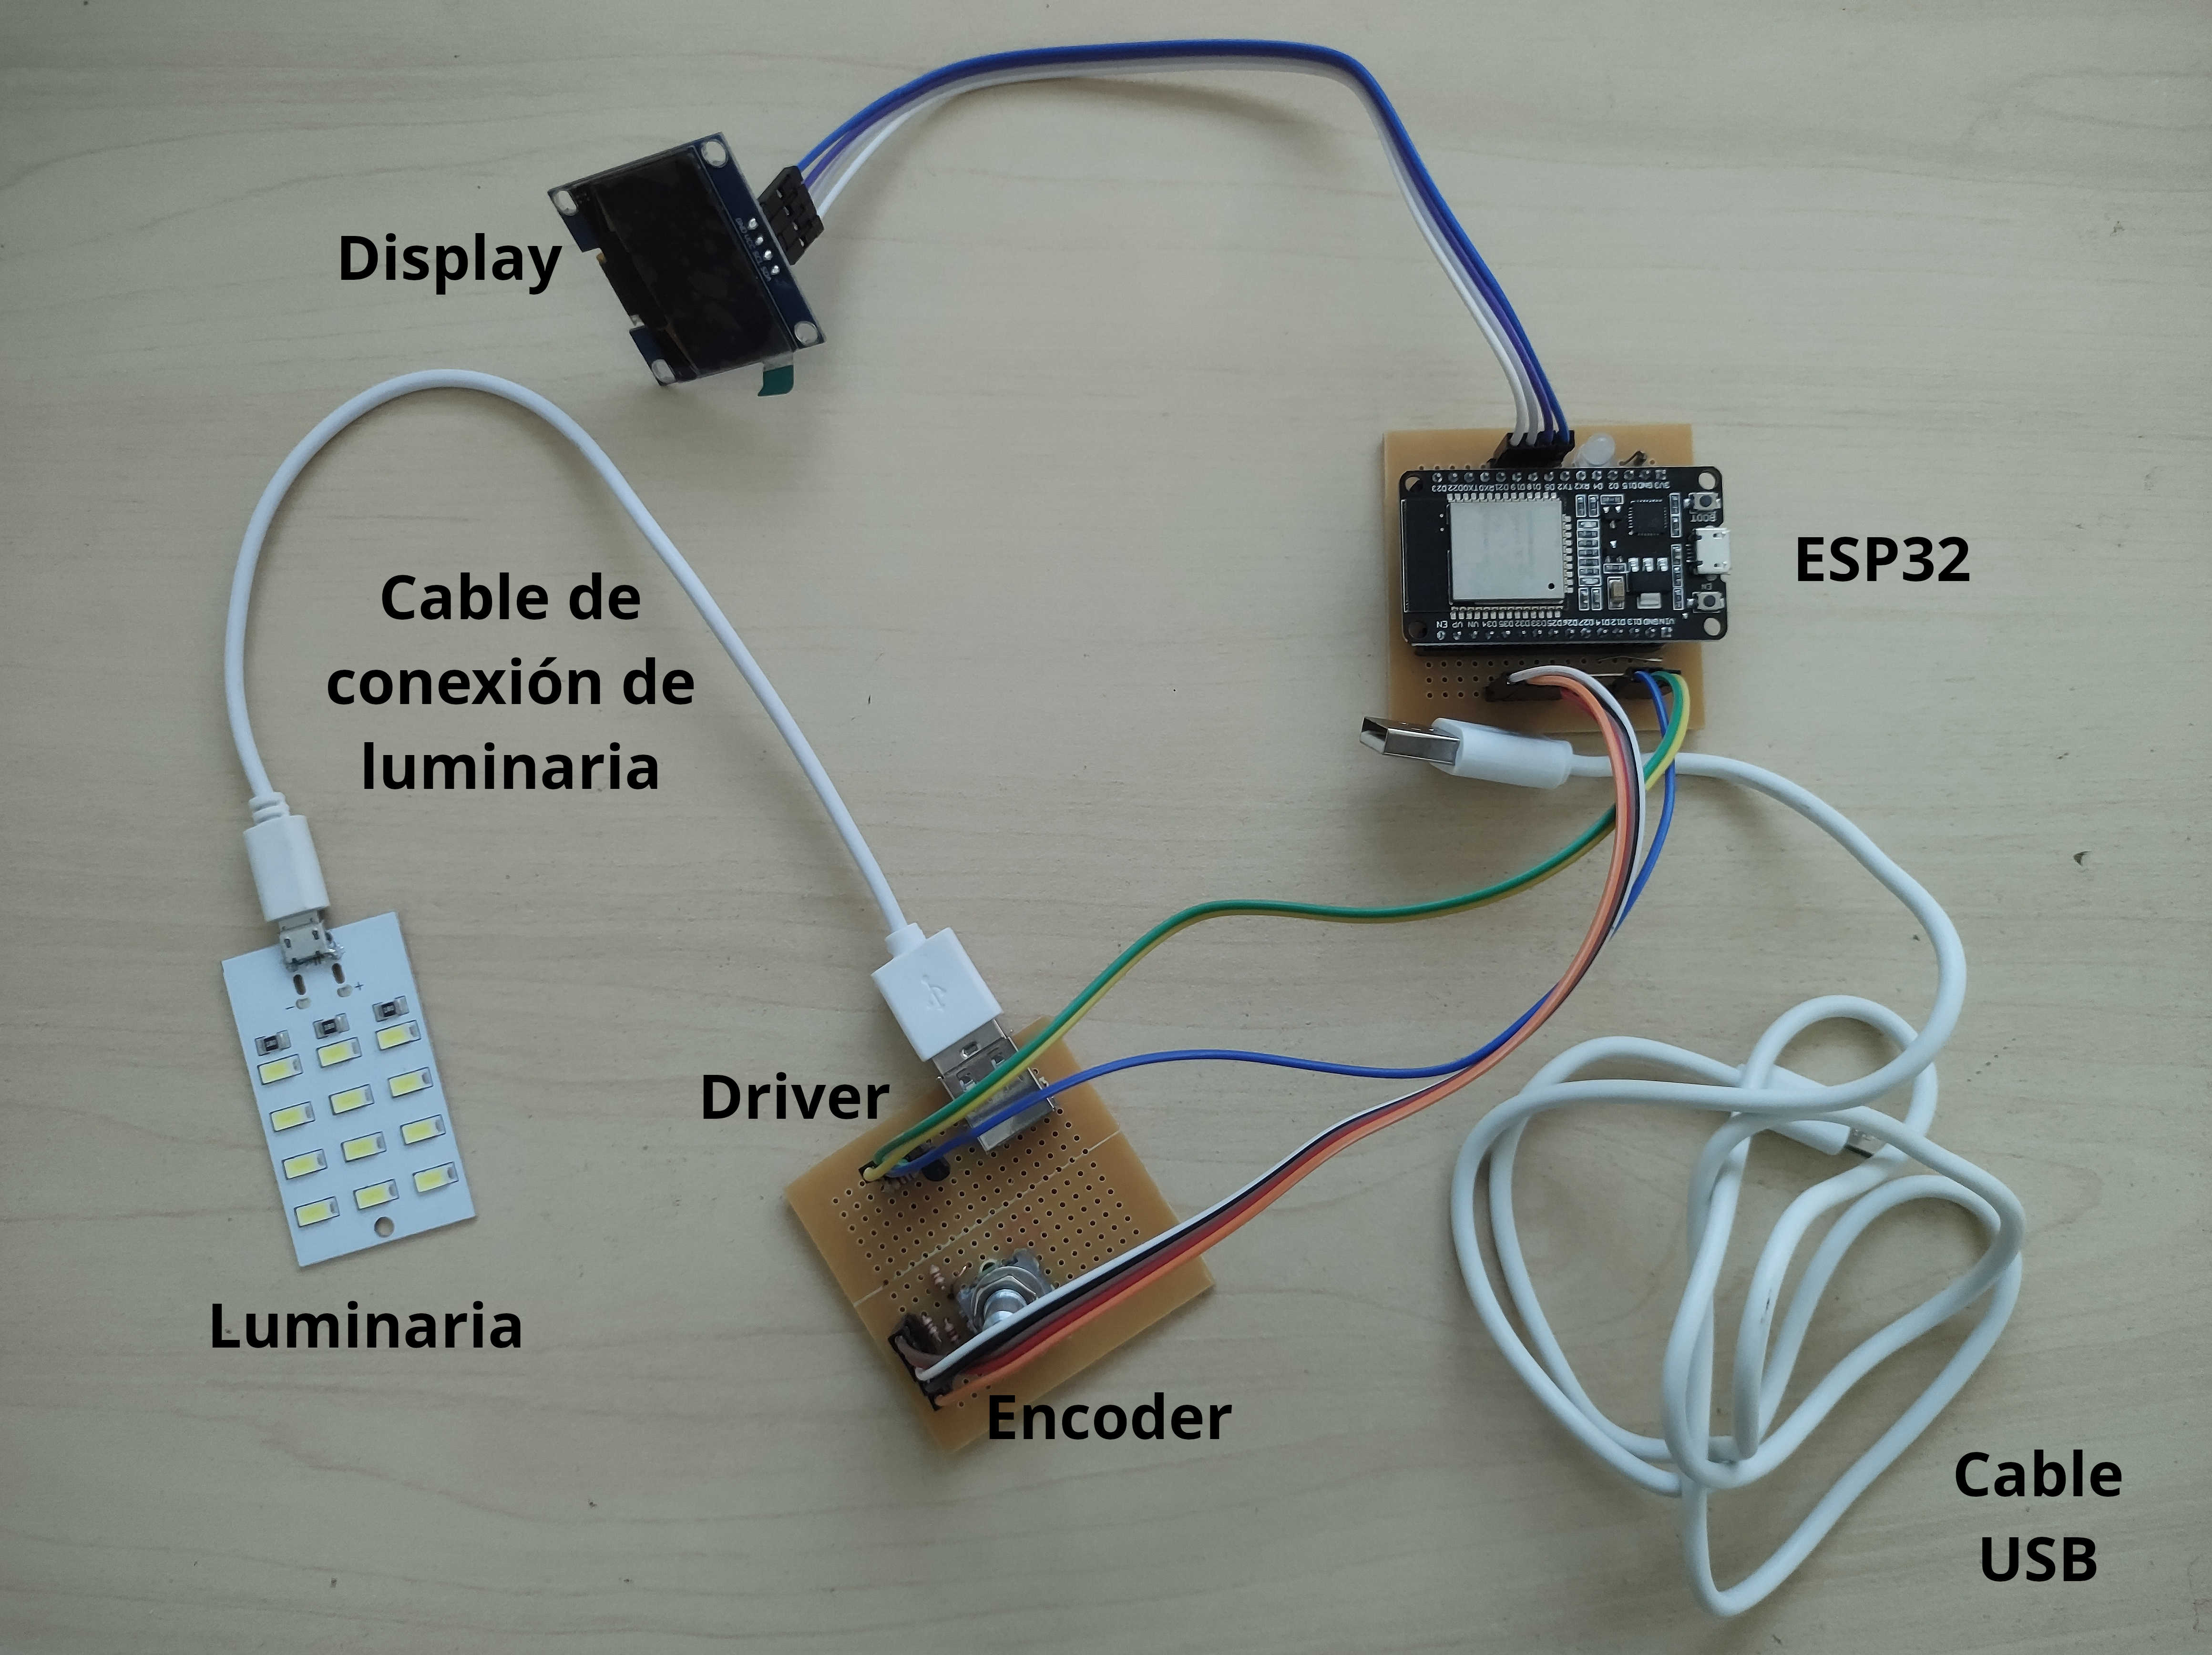
\includegraphics[scale=0.06]{Figura 32 - Nodo dimmer.jpg}
\caption[Nodo dimmer]{Componentes del nodo de dimerización.}
\label{fig:32}
\end{figure}

Se puede observar la placa ESP32 montada sobre la placa de conexiones, el display, encoder, \textit{driver} de iluminación y la placa de LEDs de 5 VCC. El control posee un conector USB por lo que puede conectarse cualquier lámpara que funcione en este caso con 5 VCC y posea este conector.

En la figura \ref{fig:33} pueden verse los componentes que forman parte del servidor.

\begin{figure}[h]
\centering
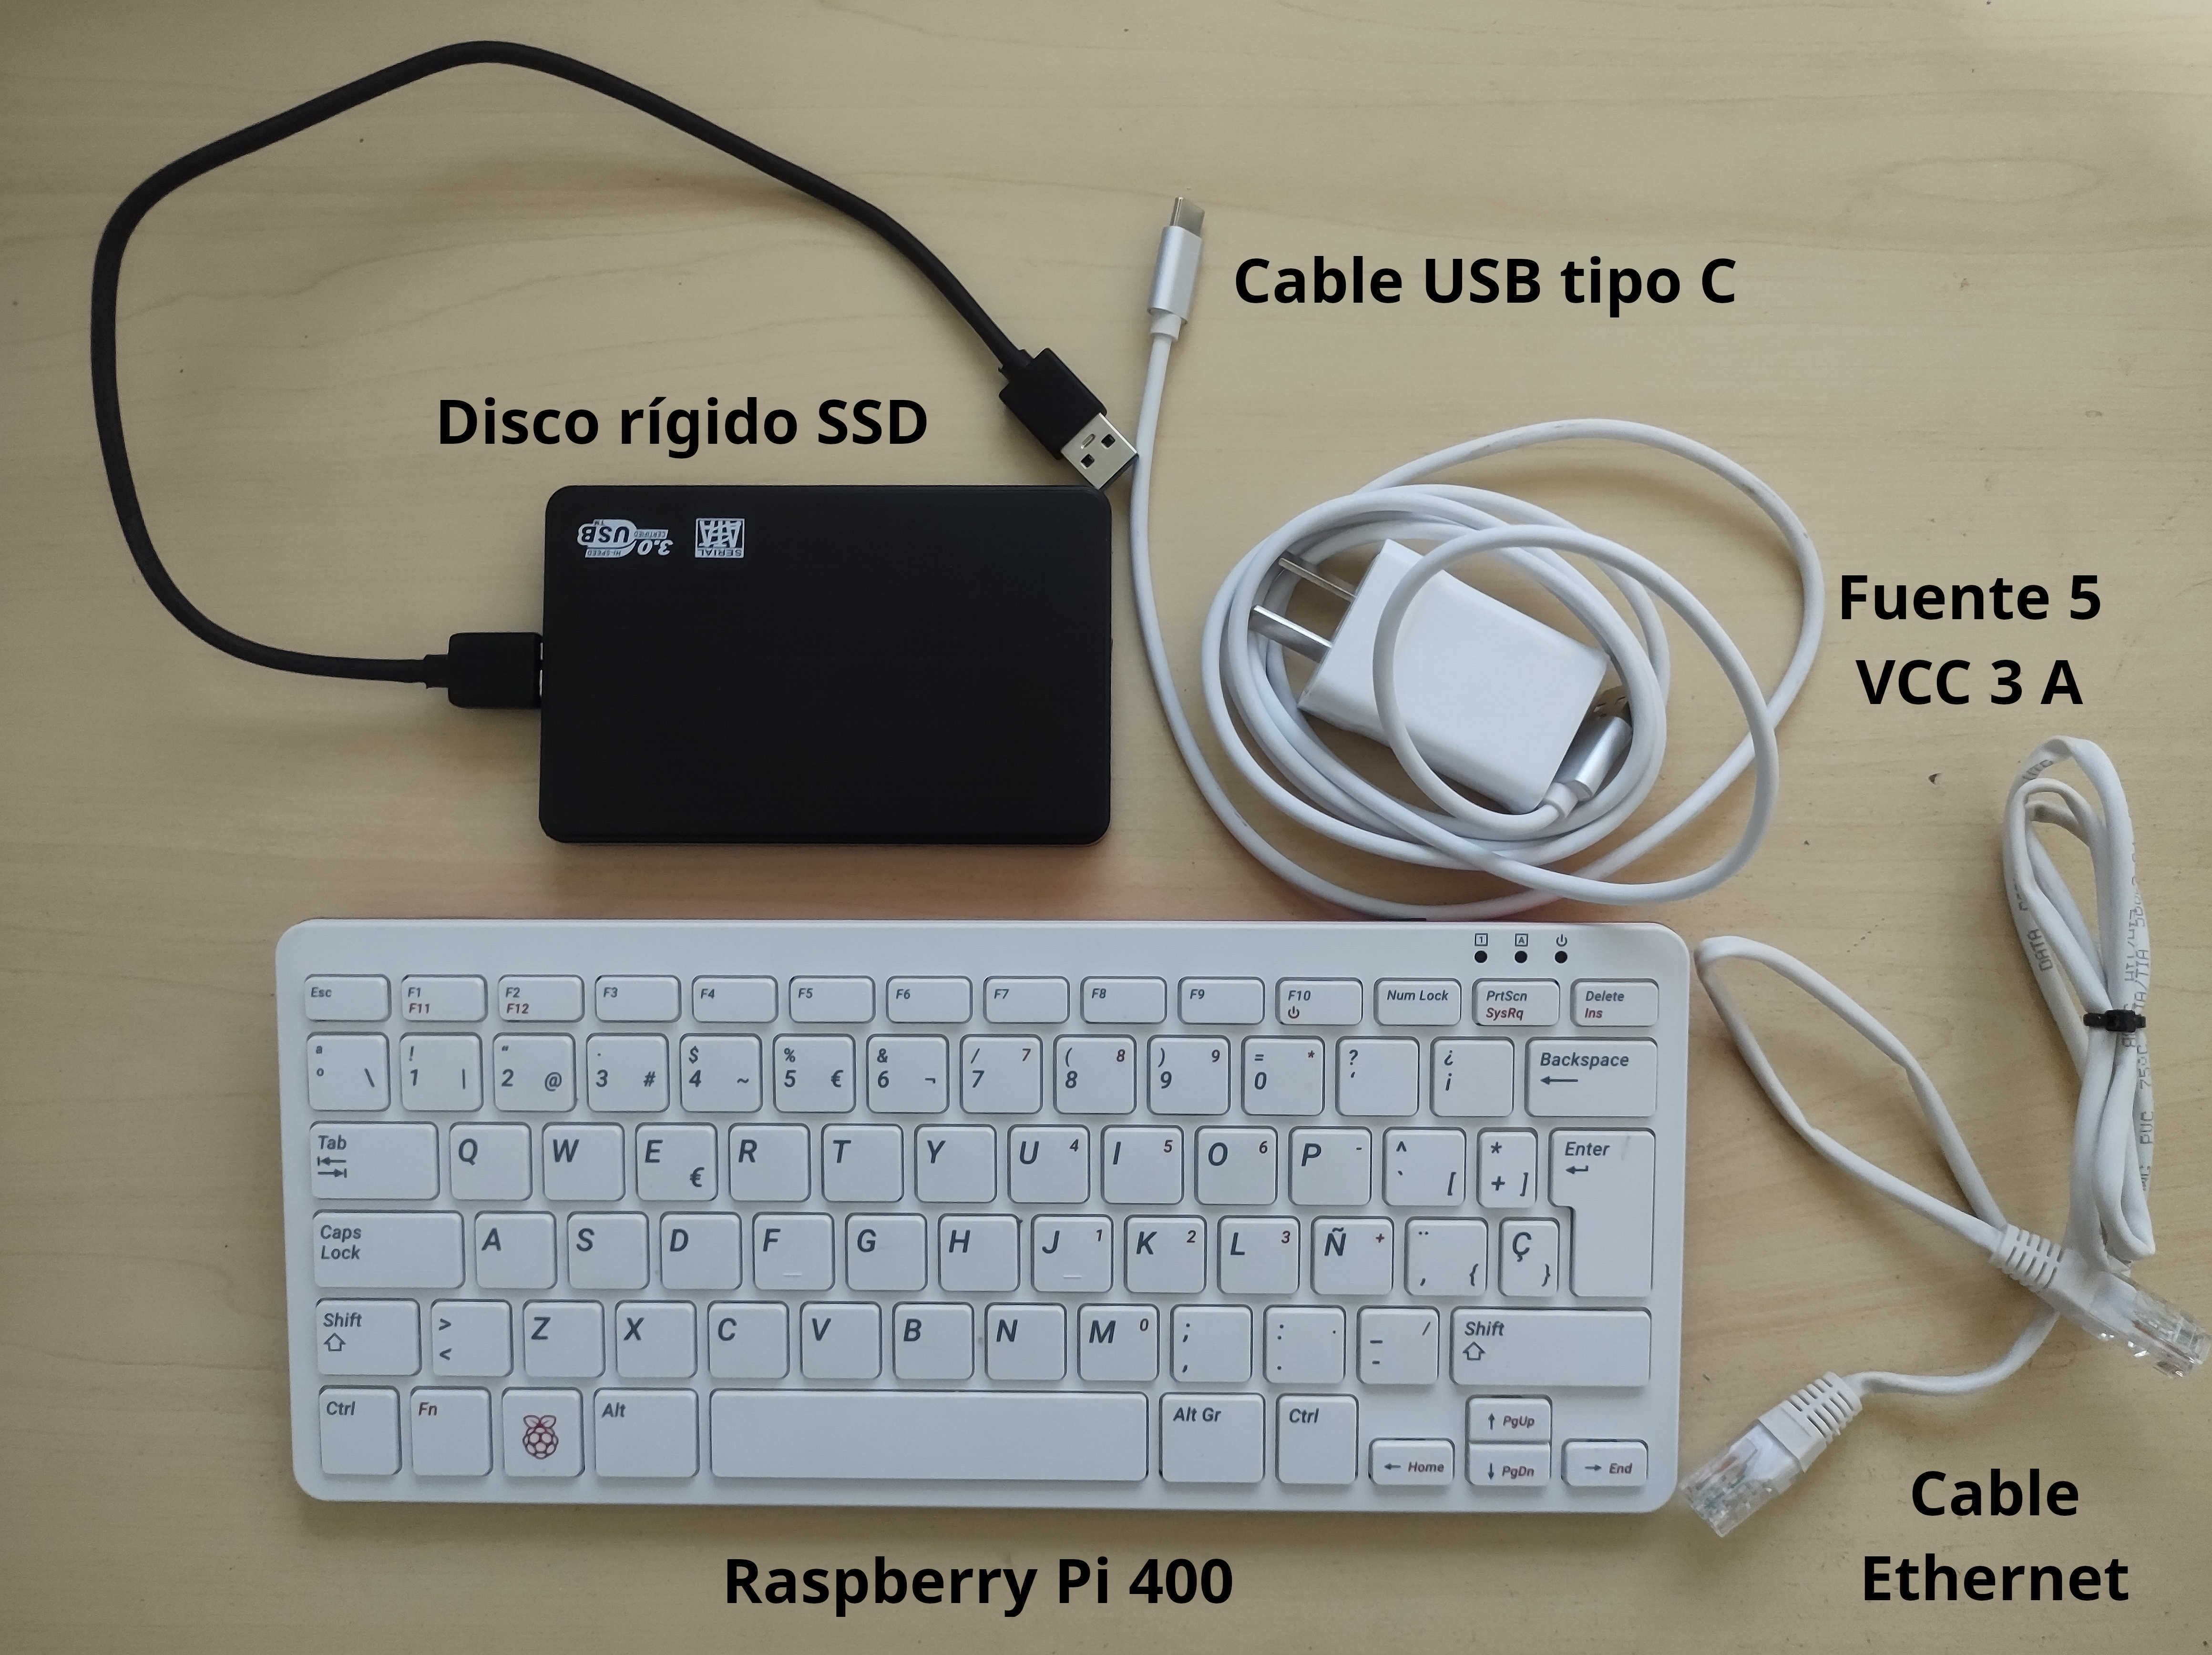
\includegraphics[scale=0.06]{Figura 33 - Servidor.jpg}
\caption[Servidor]{Componentes del servidor.}
\label{fig:33}
\end{figure}

Puede observarse la Raspberry Pi400, la fuente de 5 VCC 3A con su cable, un disco rígido externo SSD de 120 GB y un cable Ethernet para la conexión a la red.

\section{Metodología empleada}

El hardware se testeó de forma funcional. En cuanto al software se utilizaron distintas metodologías para la depuración de forma manual de los embebidos, el frontend y el backend. A continuación se describen cada una de ellas.

\subsection{Pruebas del frontend}

Para el frontend se utilizaron pruebas funcionales manuales con el sistema funcionando. Básicamente el desarrollo fue progresivo con trabajo en paralelo. Esto fue hacer una aplicación básica primero y luego seguir sumando funcionalidades. A medida que el sistema fue creciendo se fueron agregando más componentes hasta tener la versión actual.

Para las pruebas se utilizó la salida de la consola del navegador a medida que se iban implementando funciones y páginas nuevas. Con esto se logró mostrar en tiempo real el funcionamiento del sistema en cada una de las páginas y con cada función que se fue agregando. En el código \ref{lst:console front} se muestra a modo de ejemplo parte del desarrollo de la página para la visualización de un mensaje por consola de la configuración de un dispositivo.

\begin{lstlisting}[caption={Muestra por consola de los datos recibidos}, label={lst:console front}]
ngOnInit() {
    const deviceId = this.activatedRoute.snapshot.paramMap.get('id') as string;
    this.dispositivoId = deviceId, 10;
    this.subscription = this.dispositivoService.getDeviceById(this.dispositivoId).subscribe((data) => {
      console.log(data);
      this.device = data[0];
      this.tipo = data[0].tipo;
      this.ubicacion = data[0].ubicacion;
    });
    this.leerdatos();
  }
\end{lstlisting}

Allí se puede ver la función \textit{console.log} mostrando los datos por consola. En la figura \ref{fig:34} se puede ver la pantalla de configuración del dispositivo y el mensaje por consola con los datos recibidos.

\begin{figure}[h]
\centering
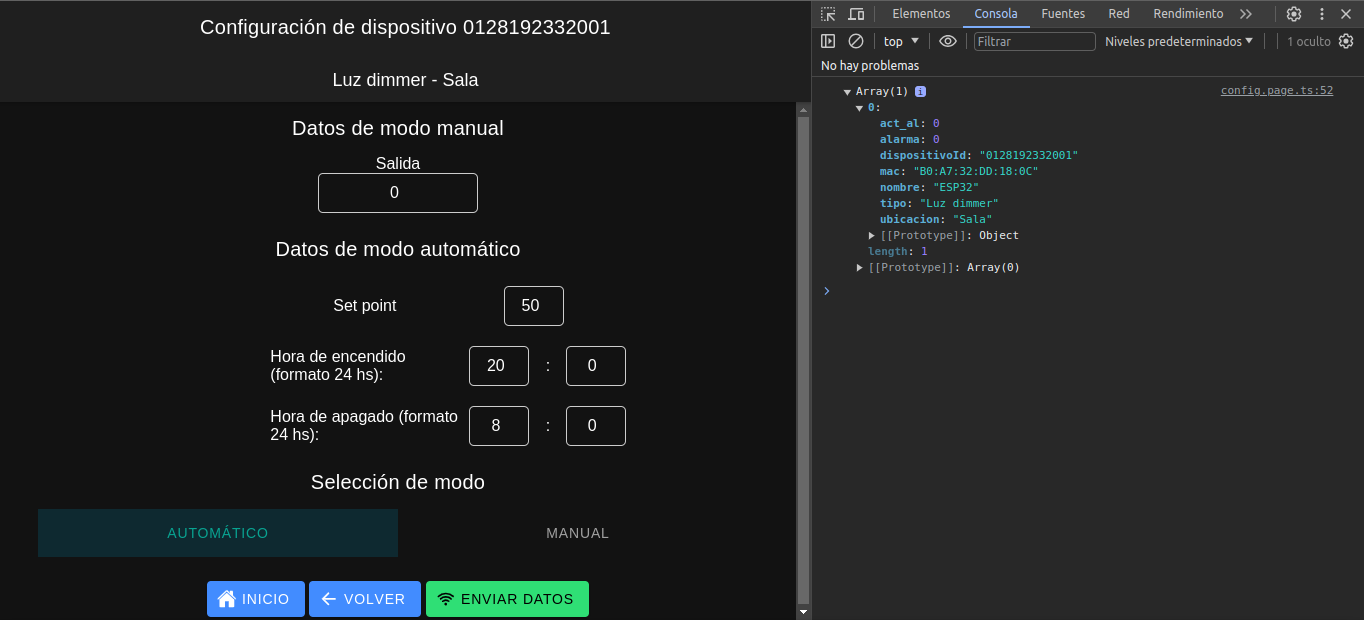
\includegraphics[scale=0.4]{Figura 34 - Consola front.png}
\caption[Prueba frontend]{Pantalla de aplicación y consola.}
\label{fig:34}
\end{figure}

Este mecanismo se utilizó en todas las páginas de la aplicación web y gracias a esto se consiguieron los resultados esperados de funcionalidad y depuración de errores.

\subsection{Pruebas del backend}

Para el backend se utilizó un mecanismo similar de pruebas funcionales que para el frontend.

El desarrollo fue progresivo por lo que a medida que se fueron incorporando funciones o endpoints nuevos, se fueron colocando muestras por consola para poder observar si los datos y las consultas estaban siendo resueltos de forma correcta. En el código \ref{lst:console back} se muestra como ejemplo el \textit{router} para borrar la tabla de mediciones de un dispositivo y el mensaje por consola de éxito y el ID del dispositivo.

\begin{lstlisting}[caption={Muestra por consola de los datos consultados}, label={lst:console back}]
borrarTablaRouter.delete('/:id', async function (req, res, next) {
  const id = req.params.id;
  let connection;
  try {
      connection = await pool.getConnection();
      await connection.beginTransaction();
      const deleteMedicionesQuery = 'DELETE FROM Mediciones WHERE dispositivoId = ?';
      await connection.query(deleteMedicionesQuery, id);
      await connection.commit();
      connection.release();
      res.send({ message: 'Mediciones eliminadas exitosamente' }).status(200);
      console.log('Solicitud de eliminacion recibida para dispositivoId:', id);
      } catch (err) {
          if (connection) {
              await connection.rollback();
              connection.release();
          }
          res.send(err).status(400);
          console.log('Error al eliminar mediciones:', err);
      }
  });
\end{lstlisting}

En la figura \ref{fig:35} se puede ver la consola con el mensaje de éxito y el ID del dispositivo cuya tabla de mediciones fue eliminada.

\begin{figure}[h]
\centering
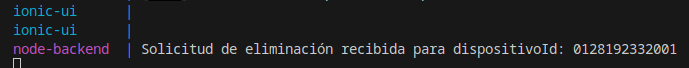
\includegraphics[scale=0.65]{Figura 35 - Consola back.png}
\caption[Prueba backend]{Mensaje por consola del servidor.}
\label{fig:35}
\end{figure}

A estas pruebas se sumó el uso de la aplicación \textit{MQTTX} para testear la comunicación con el \textit{broker} y los dispositivos, especialmente al momento de implementar la seguridad con los certificados SSL. De esta forma se ensayaron la primera conexión segura, la inserción de datos desde un dispositivo simulado, el envío de configuración desde la aplicación a los nodos y el mensaje de solicitud de configuración inicial de un nodo, entre otros.

En la figura \ref{fig:36} puede verse la configuración de \textit{MQTTX} para el envío de datos de una medición simulada en el \textit{topic \textbackslash home\textbackslash temperatura\textbackslash data} para posteriormente verificar la correcta inserción en la base de datos.

\begin{figure}[h]
\centering
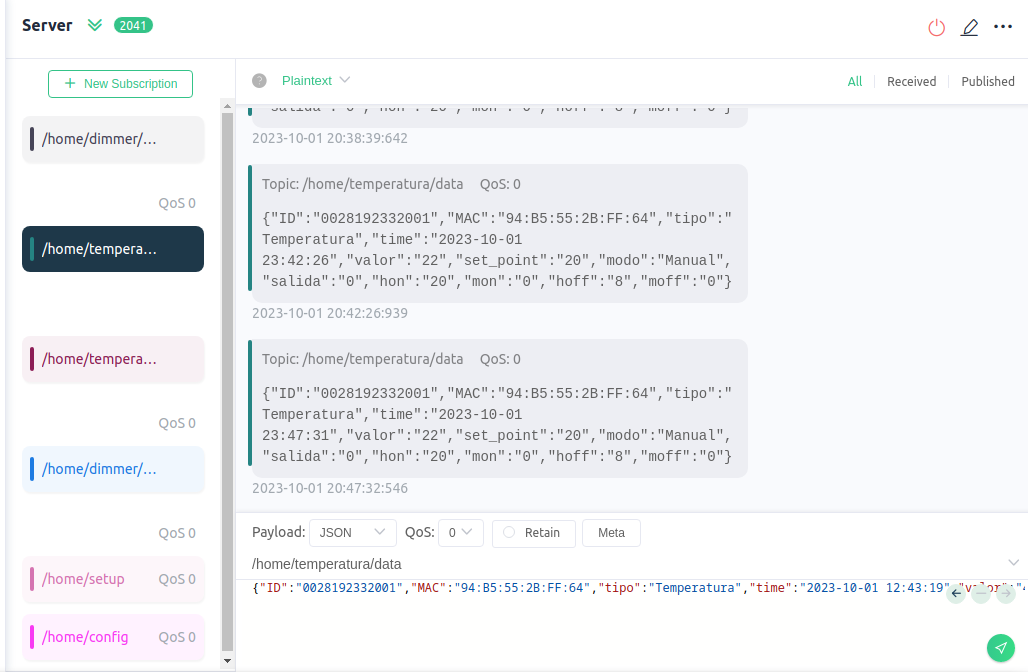
\includegraphics[scale=0.53]{Figura 36 - MQTTX.png}
\caption[MQTTX]{Pantalla de MQTTX.}
\label{fig:36}
\end{figure}

\subsection{Pruebas de los nodos}

El hardware se testeó haciendo pruebas de funcionamiento con los materiales mostrados en la sección anterior. Las pruebas constaron de hacer funcionar los nodos por dos días corridos corroborando que el control de temperatura funcione en los valores configurados y que la luminaria encienda y respete los valores de los saltos. Además se probó el funcionamiento de los horarios de encendido y apagado.

En cuanto al software, las placas ESP32 poseen comunicación serial incorporado por lo que se colocaron funciones de muestra por consola al momento de incorporar funcionalidades nuevas. En el código  \ref{lst:dispositivo} se puede observar a modo de ejemplo el uso de la función \textit{ESP\_LOGI} para mostrar por consola el valor de la salida recibido por MQTT.

\lstset{frame=tb,
  language=C++,
  aboveskip=3mm,
  belowskip=3mm,
  captionpos=b,
  showstringspaces=false,
  columns=flexible,
  basicstyle={\small\ttfamily},
  numbers=left,
  numberstyle=\tiny\color{gray},
  keywordstyle=\color{blue},
  commentstyle=\color{dkgreen},
  stringstyle=\color{mauve},
  breaklines=true,
  breakatwhitespace=true,
  tabsize=3,
}

\begin{lstlisting}[caption={Muestra por consola de la terminal ESP-IDF}, label={lst:dispositivo}]
const cJSON *salida = cJSON_GetObjectItemCaseSensitive(root, "salida");
    if (cJSON_IsNumber(salida) && select) {
        if(salida->valueint==100)
            out_temp=true;
        if(salida->valueint==0)
            out_temp=false;
        ESP_LOGI(TAG, "Received MQTT salida: %d", salida->valueint);
        pant_main();
    }
\end{lstlisting}

En este caso se muestra por consola el mensaje de recepción del valor de salida y su valor correspondiente.

\section{Resultados finales}

Como prueba final se montaron los 2 nodos, y al de temperatura se le conectó un calefactor eléctrico de 750 W. Del lado del servidor se puso a correr el \textit{docker compose} con el sistema completo. Se hicieron seteos tanto desde la aplicación web como de cada uno de los nodos.

En la figura \ref{fig:37} sel lado izquierdo se ve el nodo de iluminación funcionando encendido y en la pantalla se observa el valor de la salida y del lado derecho la pantalla de configuración de modo automático.

\begin{figure}[h]
\centering
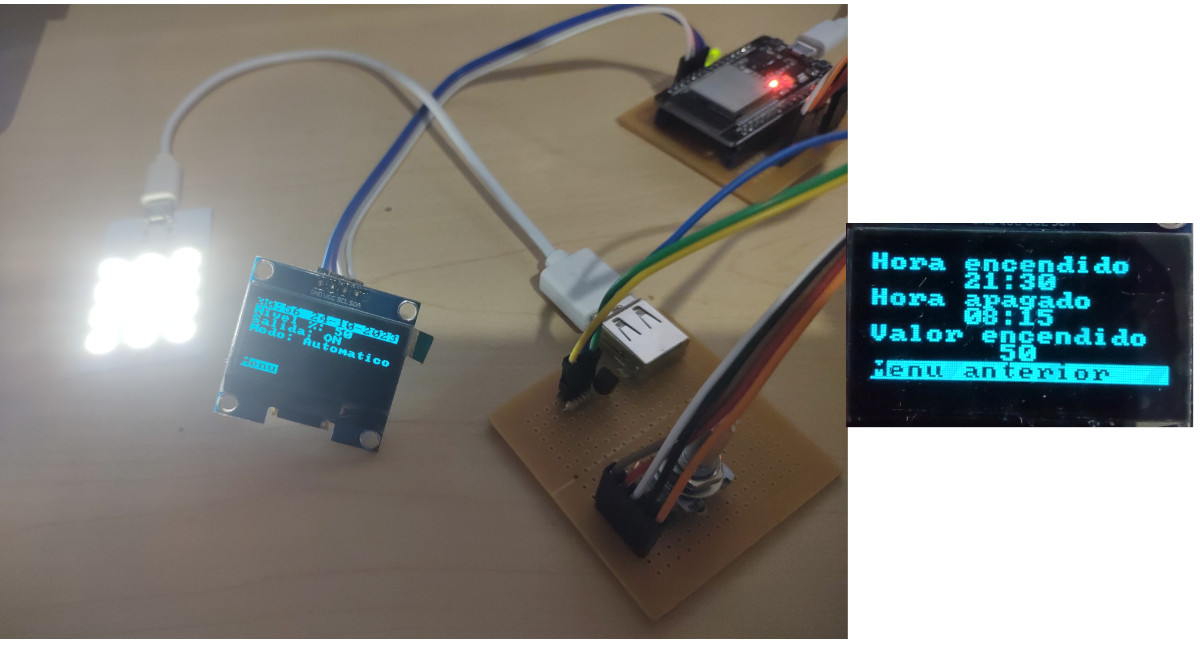
\includegraphics[scale=0.35]{Figura 37 - Dimmer funcionando.jpg}
\caption[Dimmer funciona]{Dimmer en modo automático funcionando.}
\label{fig:37}
\end{figure}

En la figura \ref{fig:38} puede observarse la página de configuración del nodo dimmer. Puede observarse que los datos ingresados corresponden con los datos guardados en el nodo y que está actuando como corresponde.

\begin{figure}[h]
\centering
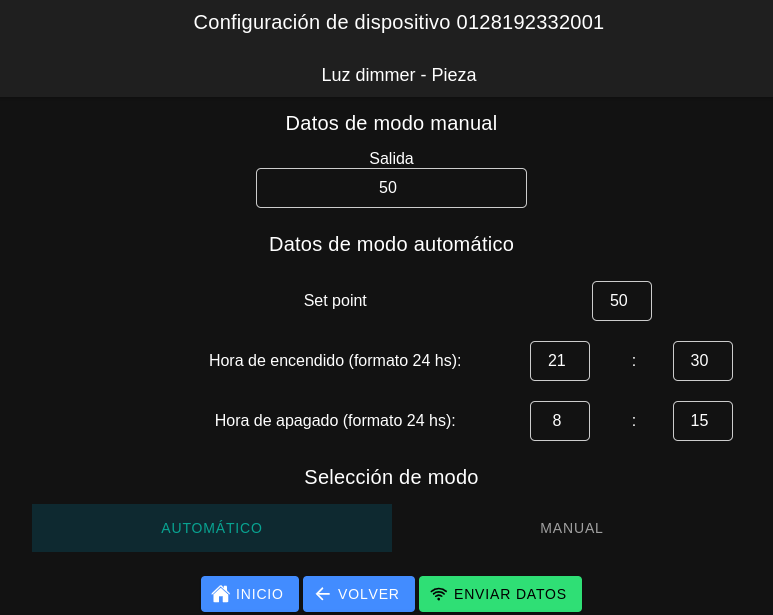
\includegraphics[scale=0.4]{Figura 38 - Config.png}
\caption[Config dimmer]{Pantalla de configuración de dimmer.}
\label{fig:38}
\end{figure}

Se corroboró que se agreguen y modifiquen los datos de los dispositivos desde la página correspondiente, comprobando con los datos que se ven en la pantalla de \textit{phpMyAdmin}. En una prueba que se realizó se cargó un dispositivo nuevo y se corroboró desde la aplicación del sistema y desde la página de administración de la base de datos. En la figura \ref{fig:39} puede verse como se agregó un dispositivo nuevo desde la página en la parte superior y como se ve reflejado en la base de datos en la inferior.

\begin{figure}[h]
\centering
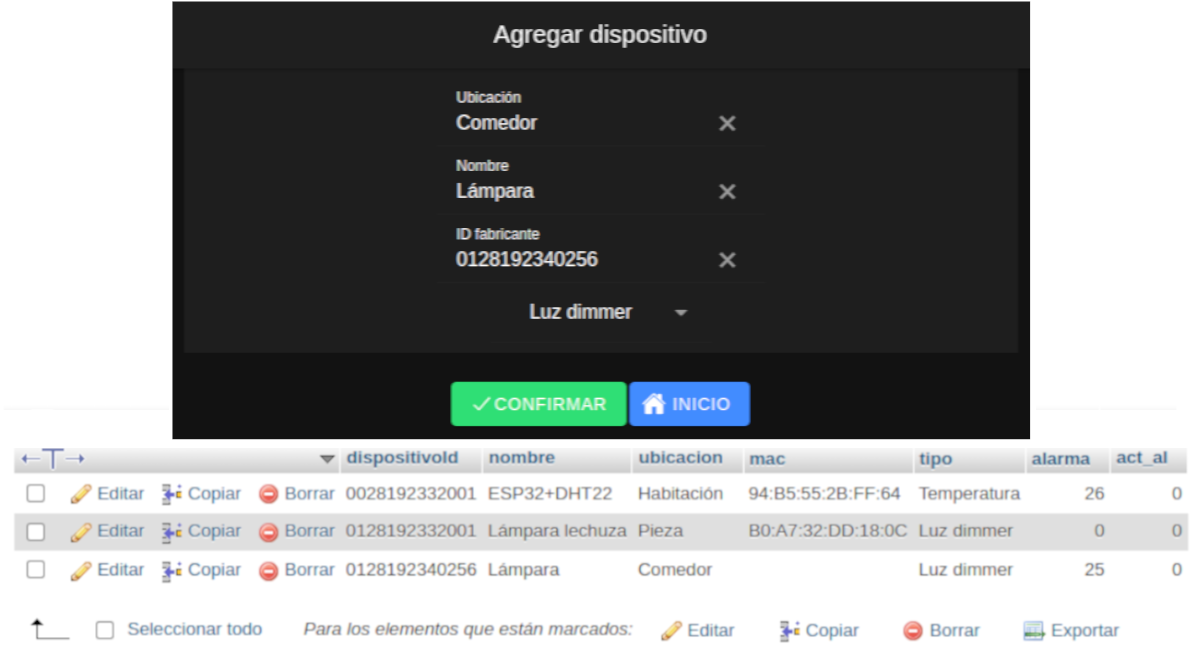
\includegraphics[scale=0.33]{Figura 39 - Agregar dispositivo.png}
\caption[Agregar dispositivo]{Valores de dispositivo nuevo.}
\label{fig:39}
\end{figure}

Puede verse que los datos cargados coinciden con los almacenados. La diferencia radica en que no se registró la MAC del dispositivo ya que al momento de obtener la imagen el dispositivo no había emitido datos al servidor.

Algo similar a la prueba de los dispositivos se hizo con los usuarios. El sistema por default tiene los valores \textit{user1}, \textit{user2} y \textit{user3} y contraseña \textit{user}. Esto se logró creando estos usuarios con sus datos en el archivo de creación de la base de datos \textit{domotica.sql}. En la figura \ref{fig:40} se muestran los valores ingresados en la página de configuración en la parte superior y los que están almacenados en la base de datos en la inferior. Como se puede observar en la imagen, los valores cargados desde la página coinciden con los almacenados en la base de datos.

\begin{figure}[h]
\centering
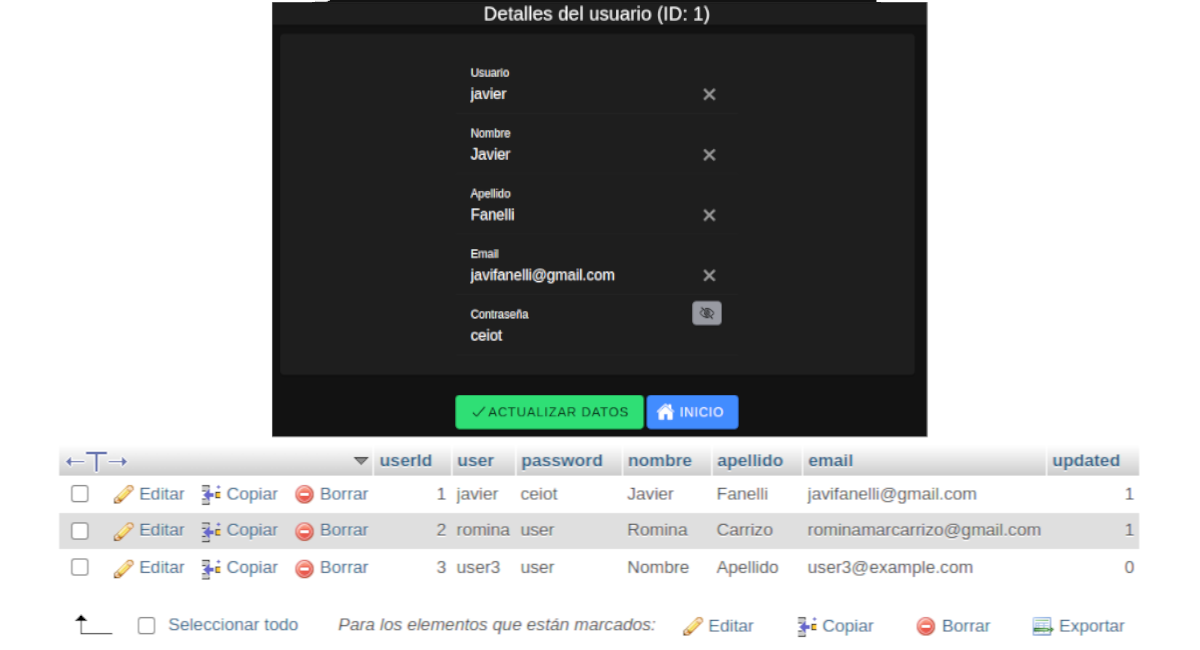
\includegraphics[scale=0.33]{Figura 40 - Modificar usuario.png}
\caption[Cambiar usuario]{Valores de usuario modificados.}
\label{fig:40}
\end{figure}

Por último se hizo la corroboración de la activación de la alarma y el envío del mail. En la figura \ref{fig:41} puede observarse la configuración del dispositivo en la parte superior y el mail recibido en la parte inferior.
\newpage
\begin{figure}[h]
\centering
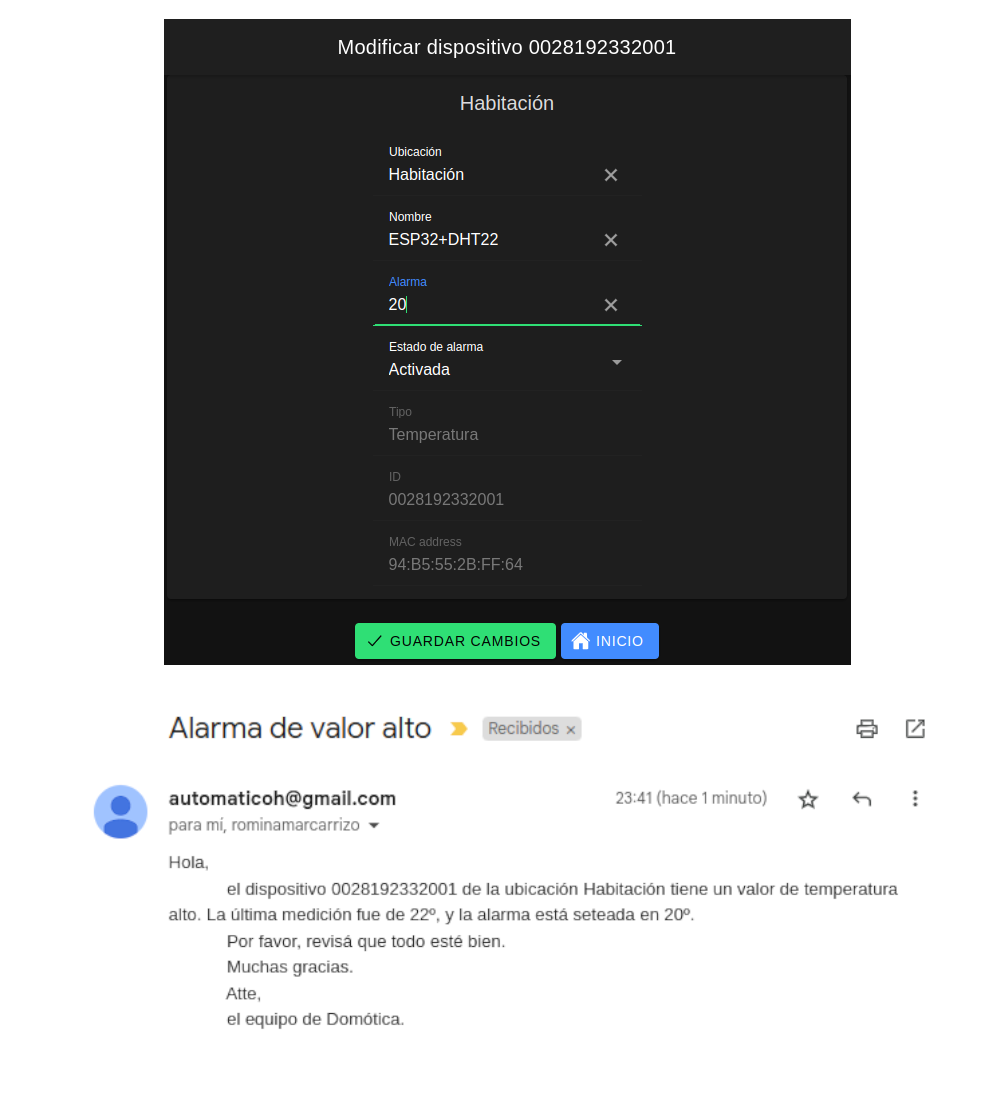
\includegraphics[scale=0.35]{Figura 41 - Alarma.png}
\caption[Cambiar usuario]{Valores de usuario modificados.}
\label{fig:41}
\end{figure}

De esta forma se hicieron las pruebas más importantes de funcionalidades del sistema. Al dar resultados de funcionamiento satisfactorios, se concluye que la aplicación funciona de manera correcta.

\section{Comparación con el estado del arte}

En la tabla \ref{tab:estadoarte} se encuentra la comparación entre las soluciones de hogares inteligentes existentes en el mercado nacional, Domotic y Reactor, y el trabajo realizado. 

\begin{table}[h]
\centering
\caption[Estado arte mercado nacional]{Comparativa entre las distintas opciones}
\begin{tabular}{l c c c}
\toprule
\textbf{Funcionalidad} & \textbf{Domotic} & \textbf{Reactor} & \textbf{Trabajo final}\\
\midrule
Posee unidad central			& Sí		& No		& Sí\\
Capacidad de diseño de		&		&		&\\
dispositivos nuevos			& Sí		& Sí		& Sí\\
Almacenamiento de mediciones	& No		& Sí		& Sí\\
Programación de reacciones	& Sí		& Sí		& Sí\\
Aplicación en ambientes		&		&		&\\
profesionales y oficinas		& No		& Sí		& Sí\\
Avisos por mail				& No		& Sí		& Sí\\
Aplicación móvil				& Sí		& Sí		& No\\
Conexión	 desde el exterior	& Sí		& Sí		& No\\
\bottomrule
\hline
\end{tabular}
\label{tab:estadoarte}
\end{table}

Como se puede observar de la tabla comparativa, el trabajo está a la altura de otras soluciones similares. Como puntos positivos, el sistema desarrollado posee una unidad central, en este caso el servidor, es capaz de aceptar diseños nuevos de dispositivos, posee avisos al suceder eventos y almacena valores de mediciones que sean útiles.

En cuanto a los aspectos a mejorar se describirán en el capítulo 5 en la sección de trabajo futuro.